\documentclass{article}
\usepackage[utf8]{inputenc}
\usepackage{amssymb}
\usepackage[margin=0.4in]{geometry}
\usepackage{natbib}
\usepackage{graphicx}
\usepackage{multicol}
\usepackage{listings}
\date{}
\usepackage{xcolor}
\usepackage{hyperref}
\hypersetup{
    colorlinks=true,
    linkcolor=blue,
}

% DURRY'S AUTOBOOTSTRAPPING NOOB CONFIGURING EXECUTABLE
\title{DANCE guide}
\author{Giovanni Durante}

\begin{document}
\maketitle
\section*{What is the purpose of DANCE}
DANCE is an automatic customization script written for those who don't want to spend their time ricing up their system. The various configurations provided here are minimal so that you can just add any feature you need without coming up with a bloated system. Ease of use is the main focus, everything should be accessible without you getting an headache. Ergonomics won't be sacrificed for the sake of aesthetics. This script is tested and currently works for the following GNU/Linux distros: Arch.

\section*{Getting started}
The installed WM is my riced version of Xmonad. After you familiarize with with default setup I suggest you you to read the config files and edit things you don't like. If, before installation, you want add some files or packages to install just edit \verb|config.yml| it's very simple to read. Added files must be put in the same directory of \verb|install.sh|

\subsection*{Keybindings}
You can use the arrow keys instead of h/j/k/l. The Mod key is the window key.
\newline Window basics \hfill System essentials
\renewcommand{\labelitemi}{\textbullet}
\renewcommand\labelitemii{\textbullet}
\begin{multicols}{2}
\begin{itemize}
    \item Mod+Enter spawn alacritty (terminal)
    \item Mod+c close window
    \item Mod+f toggle fullscreen
    \item Mod+j/k move focus to next window
    \item Mod+Shift+h/l decrease/increase border gaps
    \item Mod+Shift+j/k decrease/increase gaps
    \item Mod+n use next windowing configuration
    \item Mod+t force window back to tiling
    \item Mod+(0-9) go to workspace
    \item Mod+Shift+(0-9) move current window to that workspace
    \item Mod+Tab switch windows position
    %%\item Mod+0 open exit mode, select if you want to lock, poweroff, reboot, switch user, suspend
    \item Mod+Shift+r recompile and restart Xmonad
    \item Mod+u change keyboard layout
\end{itemize}
\hfill Basic programs
\begin{itemize}
    \item Mod+g grid view
    \item Mod+a currently running software grid
    \item Mod+d dmenu
    \item Print take a screenshot
    \item Mod+m open "dj" set
    \item Mod+s select special charaters
    \item Mod+Shift+p toggle/untoggle picom
    \item F12 open drop down terminal, also to open/close the "dj" set
\end{itemize}
\end{multicols}

\section*{Stuff to be configured manually}
If you are using a laptop you might want to spend some time setting up hardware accelleration to improve battery life, refer to your distro documentation \footnote{Arch docs are always very useful! \href{https://wiki.archlinux.org/index.php/Hardware_video_acceleration}{HW accel} also for \href{https://wiki.archlinux.org/index.php/chromium#Hardware_video_acceleration}{chromium} and \href{https://trac.ffmpeg.org/wiki/HWAccelIntro}{FFmpeg}}. In order to use cmus (music player) you need to run it and specify where to search for music with \verb|:add ~/path/to/dir/|. Replace \verb|wlp2s0| with your network card name (ip addr) in \verb|~/.xmonad/scripts/status-net|.

\section*{Images}

\begin{figure}[h!]
    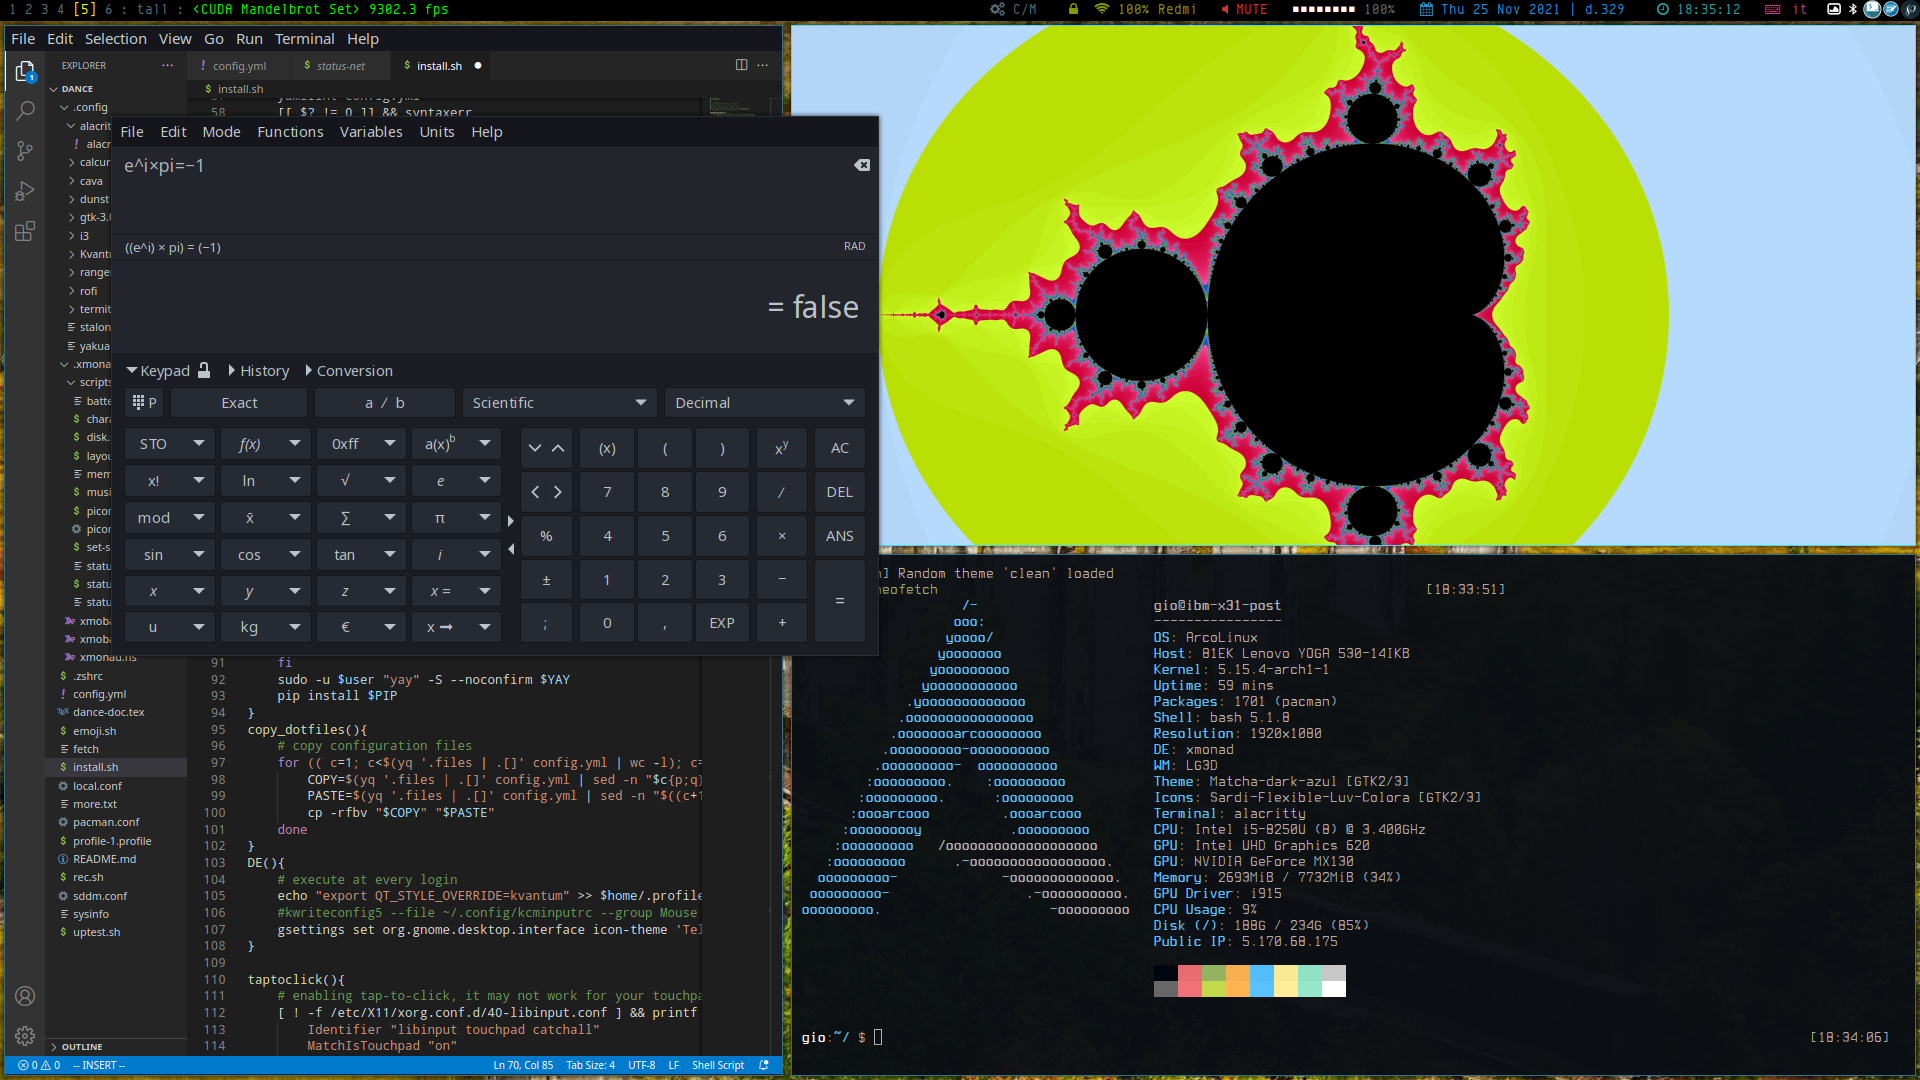
\includegraphics[width=19.3cm]{dance_prew2.png}
    \newline
    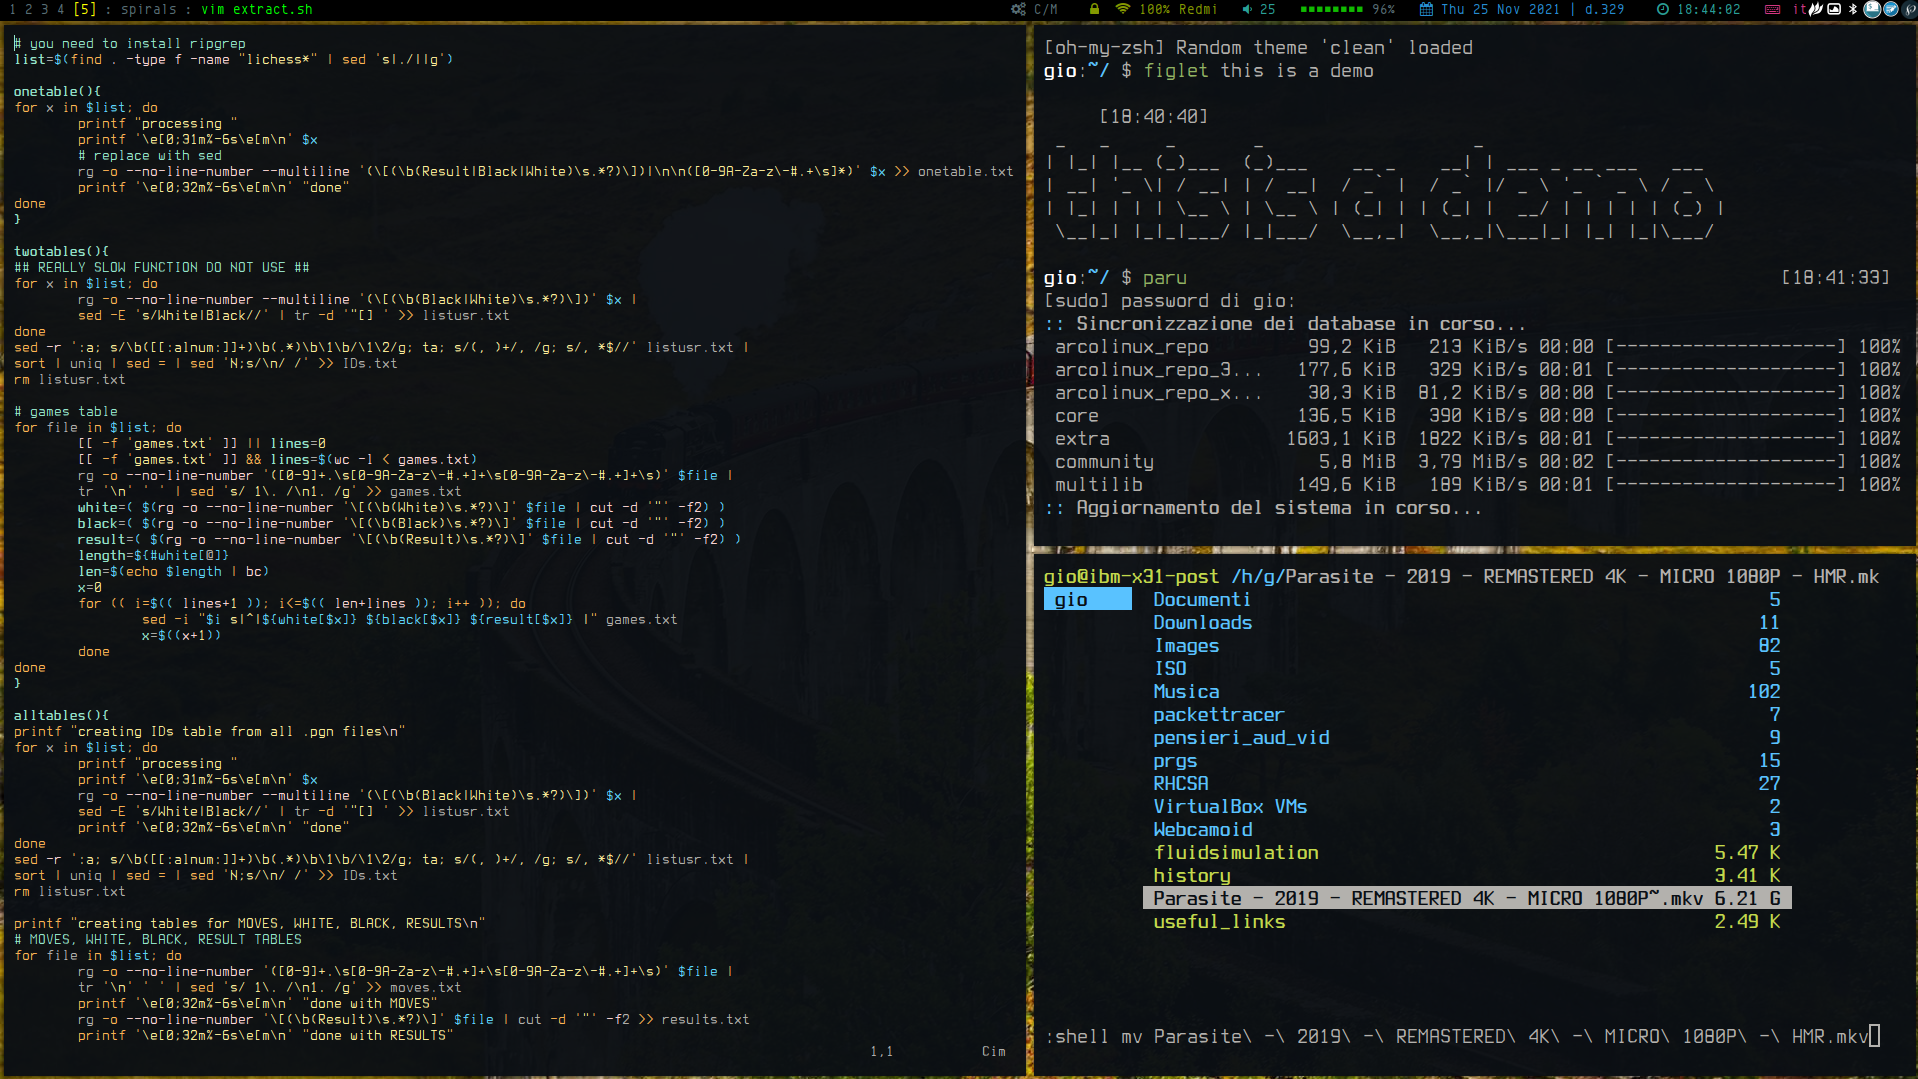
\includegraphics[width=19.3cm]{dance_prew3.png}
    \newline
\end{figure}

\section*{Contact me! plz}
\href{mailto:giovanni3durante@gmail.com}{giovanni3durante@gmail.com} | Email me!
\newline
\href{https://github.com/durryx}{My Github}
\newline
\href{https://www.paypal.com/paypalme/durrysas}{Paypal}

\end{document}
